\section{Versioned Correspondence Between the Two Studies}
\label{app:correspondence}
\begin{table*}[t]
\centering\small
\setlength{\tabcolsep}{4pt}
\renewcommand{\arraystretch}{1.09}
\begin{tabularx}{\textwidth}{@{}>{\raggedright\arraybackslash}p{.17\textwidth}>{\raggedright\arraybackslash}X>{\raggedright\arraybackslash}X@{}}
\toprule
Binding & Study A: theft-method-freeze/5.0.0 & Study B: native-150 compact controller \\
\midrule
Knowledge & Source-extracted propositions, macro graph, refined local evidence rules and mapped routes & Common deterministic compilation of all three public tenancy templates \\
Online gate & Rule-local true/false/unresolved guard; macro edges do not gate requests & Inherited applicability scopes, obligation condition and separate acquisition permission \\
Evidence state & Held document types; true-guard confirmation; union of mapped routes & Presence, capability/route adequacy, multi-document joint adequacy; per-capability route selection \\
State update & Recompute requests/next action from a changed packet; paired edit, not acquired evidence outcome & Recompute from a new assessment; benchmark measures one planning realization \\
Population & 9 development + 27 held-out pairs; nine shared concepts, four contexts; 72 units total & 60 development/11 families + 90 protected/17 families; 150 claims, three tenancy domains \\
Learned inference & Guard-major batched V5; 1-call Direct, 1-call representation baseline, 2-call Evidence-first & Five 2-call singleton pipelines; two additional controls reuse CasePath state \\
Endpoint & Route-aware signed additions/withdrawals, 27-pair micro scores & Complete native artifact and separate actual immediate-checklist metrics \\
Analysis & Historical family bootstrap, exact family swaps and wrong-family diagnostic; broad gate failed & Equal domain/family/case finite contrasts; family-deletion sensitivity, no significance claim \\
Parity & Recorded-answer replay over 72 units and 36 deltas & Separate implementation; no inherited V5 or six-role/live-app parity claim \\
\bottomrule
\end{tabularx}
\caption{A common source-to-state-to-evidence interface does not make the two
implementations, populations or measurements interchangeable. Study B extends
the evidence question rather than retrospectively re-evaluating V5.}
\label{tab:full-correspondence}
\end{table*}


The shared interface is source specification, case assessment, evidence
planning, state replacement and a justified next action. It does not assert
identical knowledge, algorithms, estimands or validation across the two
implementations. Study~A is bound to
\path{casepath.theft-method-freeze/5.0.0}, interpreter V4 and evidence
overlay V3; Study~B is bound to the compact native producer and its
\texttt{obligation\_control\_v1} and \texttt{evidence\_demand\_v1}
controller. The native public template union is not a transfer of the theft
source pack, and the theft pairs are not transformations of the native claim
roster. V5 judges local guards and projects every mapped route on active
rules plus mapped confirmation evidence for true unconfirmed guards, minus
held document types; it implements neither capability-specific nor joint
adequacy. The native controller distinguishes applicability from
acquisition, unknown from missing evidence, and per-capability route
selection from route union. These are substantive version differences, and
no benchmark comparison between the runtimes is claimed. Study~A's
preparation extracted propositions, synthesised and refined rules and mapped
capabilities with model calls and retained source-only corrections; its
reported held-out costs exclude that preparation. Study~B's compilation is
deterministic and shared by all arms.

\section{Study B: Native Measurements and Analysis Contract}
\label{app:native-metrics}

\paragraph{Native endpoints.}
Native critical-evidence recall is criticality-weighted coverage of active
evidence obligations through any complete permitted document alternative.
Evidence-obligation completeness additionally requires valid
decision--fact--capability--document relations. Valid-chain precision counts
requested items with such a chain over all requested items; its empty-set
value is one and must be read beside coverage. Wrong-branch and premature
requests, document states, node and edge scores, branch and path probes and
source locators retain their native contracts; locator agreement is not
semantic entailment, and probe accuracy is not a direct measure of inferred
case-predicate accuracy. The emitted endpoint counts unique immediate
request identities without activating candidate conditions from the
reference scenario, and is available only when the reference has a unique
allowed document set for every active obligation, complete consistent
document states and the public label mapping. For predicted and reference
sets $P,G$: $F_1=2|P\cap G|/(|P|+|G|)$ and unnecessary fraction
$U=|P\setminus G|/|P|$; both-empty $F_1$, empty-prediction precision and
empty-reference recall are one, and empty-prediction burden is zero. Failed
cells use adverse frozen unit penalties instead: zero for higher-is-better
rates, one for lower-is-better rates. Unavailable reference labels never
become empty sets or silently shrink a denominator.

\paragraph{Estimation.}
For a split or the complete corpus, each scheduled case has weight
$\omega_i=1/(3\,m_{d(i)}\,n_{f(i)})$, where $m_d$ is its domain's family
count and $n_f$ its family's scheduled case count. Conventional differences
use adverse-imputed unit scores; conservative benefit-oriented differences
contribute $-1$ whenever either producer endpoint is unobserved. Every
single-family deletion is reported with remaining weights renormalised
within the affected domain; these ranges are composition sensitivity, not
confidence intervals. A comparator is counted as beaten only when all three
conservative contrasts strictly exceed their boundaries on the complete
protected population under the original references and integrity checks;
otherwise the report labels the outcome as not met, a partial practical
signal, or not evaluable.

\paragraph{Execution and failure classes.}
Each cell records its arm, case, state and either the validated artefact or
the retained provider output with the reason validation failed. Unknown
relation endpoint: a candidate artefact relation references a node identity
that does not exist in the artefact. Truncated or non-terminal: the
completion reached the \nbTokens-token limit or ended without a terminal
outcome. Invalid codebook index: a reference into the shared public codebook
that does not resolve. Contradictory presence state: a document marked both
present and absent, or present with an inconsistent state. Blocked
dependency: a dependent control whose \casepath source cell failed. Every
failure retains its charge; a repaired version can never replace a failed
cell in the frozen comparison.

\section{Post-hoc Request-Only Diagnostic}
\label{app:request-diagnostic}

The registered wrapper scores emitted requests only after a native receipt
has no evaluation failures. A common expression-namespace mismatch therefore
suppresses request scoring for every generated artefact. The post-hoc
diagnostic changes that availability rule alone: it reads the unchanged
\texttt{request\_mode=now} items, maps their labels with the original public
mapping, and applies the original emitted-set scorer. It never evaluates a
candidate condition against a reference state. All original artefacts,
producer failures, native failures, primary penalties and costs remain
separately available.

All \nbClaims{} references yield an eligible unique document set. The
\nrRequestObserved{} generated lists receive observed request-only scores;
\nrRequestPenalties{} failed or blocked outputs receive the original adverse
checklist penalties, with no invented requests. Domain--family--case
weighting is unchanged. For benefit direction $b_m\in\{-1,1\}$, the
conventional paired contribution is
$b_m(s_{i,\mathrm{CP},m}-s_{i,a,m})$; the conservative contribution is the
same quantity when both request-only endpoints are observed and $-1$
otherwise. A graph's native failure does not make an independently scoreable
request list unobserved in this diagnostic. No practical threshold,
significance test or confidence interval is applied.

\begin{table}[htb]
\centering\small
\setlength{\tabcolsep}{4pt}
\begin{tabular}{lrrrrrr}
\toprule
\multicolumn{7}{l}{\textbf{Development: 60 claims}} \\
Pipeline & Lists & Correct/req. & Missed & Cond. & Prec. & Recall \\
\midrule
\casepath & \rqDevCpN & \rqDevCpCorrect/\rqDevCpRequested & \rqDevCpMissed & \rqDevCpConditional & \rqDevCpP & \rqDevCpR \\
Direct & \rqDevDirN & \rqDevDirCorrect/\rqDevDirRequested & \rqDevDirMissed & \rqDevDirConditional & \rqDevDirP & \rqDevDirR \\
Document-first & \rqDevDocN & \rqDevDocCorrect/\rqDevDocRequested & \rqDevDocMissed & \rqDevDocConditional & \rqDevDocP & \rqDevDocR \\
Process-context & \rqDevPcN & \rqDevPcCorrect/\rqDevPcRequested & \rqDevPcMissed & \rqDevPcConditional & \rqDevPcP & \rqDevPcR \\
Rule-first & \rqDevRfN & \rqDevRfCorrect/\rqDevRfRequested & \rqDevRfMissed & \rqDevRfConditional & \rqDevRfP & \rqDevRfR \\
Compiled equivalent & \rqDevCeN & \rqDevCeCorrect/\rqDevCeRequested & \rqDevCeMissed & \rqDevCeConditional & \rqDevCeP & \rqDevCeR \\
Local-scope ablation & \rqDevLsN & \rqDevLsCorrect/\rqDevLsRequested & \rqDevLsMissed & \rqDevLsConditional & \rqDevLsP & \rqDevLsR \\
\bottomrule
\end{tabular}
\par\medskip
\begin{tabular}{lrrrrrr}
\toprule
\multicolumn{7}{l}{\textbf{Protected families: 90 claims}} \\
Pipeline & Lists & Correct/req. & Missed & Cond. & Prec. & Recall \\
\midrule
\casepath & \rqHidCpN & \rqHidCpCorrect/\rqHidCpRequested & \rqHidCpMissed & \rqHidCpConditional & \rqHidCpP & \rqHidCpR \\
Direct & \rqHidDirN & \rqHidDirCorrect/\rqHidDirRequested & \rqHidDirMissed & \rqHidDirConditional & \rqHidDirP & \rqHidDirR \\
Document-first & \rqHidDocN & \rqHidDocCorrect/\rqHidDocRequested & \rqHidDocMissed & \rqHidDocConditional & \rqHidDocP & \rqHidDocR \\
Process-context & \rqHidPcN & \rqHidPcCorrect/\rqHidPcRequested & \rqHidPcMissed & \rqHidPcConditional & \rqHidPcP & \rqHidPcR \\
Rule-first & \rqHidRfN & \rqHidRfCorrect/\rqHidRfRequested & \rqHidRfMissed & \rqHidRfConditional & \rqHidRfP & \rqHidRfR \\
Compiled equivalent & \rqHidCeN & \rqHidCeCorrect/\rqHidCeRequested & \rqHidCeMissed & \rqHidCeConditional & \rqHidCeP & \rqHidCeR \\
Local-scope ablation & \rqHidLsN & \rqHidLsCorrect/\rqHidLsRequested & \rqHidLsMissed & \rqHidLsConditional & \rqHidLsP & \rqHidLsR \\
\bottomrule
\end{tabular}
\par\medskip
\begin{tabular}{lrrrrrr}
\toprule
\multicolumn{7}{l}{\textbf{Combined: 150 claims}} \\
Pipeline & Lists & Correct/req. & Missed & Cond. & Prec. & Recall \\
\midrule
\casepath & \rqAllCpN & \rqAllCpCorrect/\rqAllCpRequested & \rqAllCpMissed & \rqAllCpConditional & \rqAllCpP & \rqAllCpR \\
Direct & \rqAllDirN & \rqAllDirCorrect/\rqAllDirRequested & \rqAllDirMissed & \rqAllDirConditional & \rqAllDirP & \rqAllDirR \\
Document-first & \rqAllDocN & \rqAllDocCorrect/\rqAllDocRequested & \rqAllDocMissed & \rqAllDocConditional & \rqAllDocP & \rqAllDocR \\
Process-context & \rqAllPcN & \rqAllPcCorrect/\rqAllPcRequested & \rqAllPcMissed & \rqAllPcConditional & \rqAllPcP & \rqAllPcR \\
Rule-first & \rqAllRfN & \rqAllRfCorrect/\rqAllRfRequested & \rqAllRfMissed & \rqAllRfConditional & \rqAllRfP & \rqAllRfR \\
Compiled equivalent & \rqAllCeN & \rqAllCeCorrect/\rqAllCeRequested & \rqAllCeMissed & \rqAllCeConditional & \rqAllCeP & \rqAllCeR \\
Local-scope ablation & \rqAllLsN & \rqAllLsCorrect/\rqAllLsRequested & \rqAllLsMissed & \rqAllLsConditional & \rqAllLsP & \rqAllLsR \\
\bottomrule
\end{tabular}
\par\medskip

\caption{\textbf{Request counts and coverage.} Lists counts the generated
artefacts that contribute raw counts. Correct/req., Missed and Cond. sum only
those artefacts; Cond. counts documents deferred conditionally, not immediate
requests. Precision and recall are full-population, failure-penalized weighted
scores, and therefore differ from the ratios of the displayed raw counts.
Dependent controls reuse the same assessments.}
\label{tab:native-counts}
\end{table}

\begin{table}[htb]
\centering\small
\begin{tabular}{llrr}
\toprule
Comparator & Endpoint & Conventional & Conservative \\
\midrule
Direct & $F_1$ & \rqHidDDirF & \rqHidCDirF \\
Direct & Unnecessary fraction & \rqHidDDirU & \rqHidCDirU \\
Document-first & $F_1$ & \rqHidDDocF & \rqHidCDocF \\
Document-first & Unnecessary fraction & \rqHidDDocU & \rqHidCDocU \\
Process-context & $F_1$ & \rqHidDPcF & \rqHidCPcF \\
Process-context & Unnecessary fraction & \rqHidDPcU & \rqHidCPcU \\
Rule-first & $F_1$ & \rqHidDRfF & \rqHidCRfF \\
Rule-first & Unnecessary fraction & \rqHidDRfU & \rqHidCRfU \\
\bottomrule
\end{tabular}

\caption{Protected-family paired request-only contrasts. Positive values
favor \casepath; the unnecessary-fraction difference reverses its sign so
that less burden is positive. The conservative rule assigns $-1$ when either
endpoint is unobserved. All endpoint contrasts, all families and every
family-deletion result are included in the machine-readable report.}
\label{tab:native-contrasts}
\end{table}

\paragraph{The boundary is semantic, not just syntactic.}
The public compiler introduces \nrNativeSymbols{} condition symbols shared
by all arms. None of the emitted symbols lies outside that namespace. The
native expression language evaluates them against the contract's scenario,
which does not provide the needed assignment. An authored, target-blind
counterexample makes the difference explicit: the product controller returns
unresolved for an absent condition; the native parser raises a missing-variable
error. Assigning null instead makes the native Boolean evaluation false,
while the controller still returns unresolved. Without a public state
correspondence, a rename, default or injected predicted state would change
meaning. No such correction is made.

\begin{figure}[htb]
\centering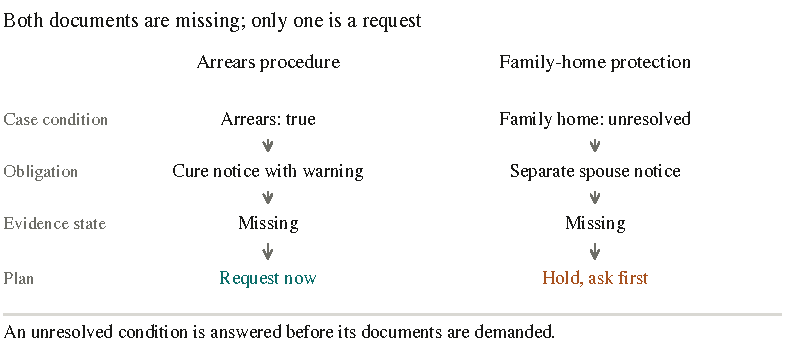
\includegraphics[width=.85\linewidth]{fig_native_case.pdf}
\caption{\textbf{A recorded controller decision.} In the first completed
\casepath development case in sorted cohort order, arrears is true and
family-home status unresolved. The cure notice is requested now; the spouse
notice remains conditional. This shows two routes within the recorded plan,
not an accepted native graph: its exported predicate namespace encounters the
same interface failure as the other generated artefacts. The release includes
the complete case trace and selection rule.}
\label{fig:native-case}
\end{figure}

\paragraph{Execution evidence and historical access.}
The primary scoring task authenticates both complete prediction inventories
before reading references. The original producer terminated without its
complete I/O audit; historical non-access to protected targets is therefore
not established retrospectively. Scoring, the compatibility diagnosis and
the request-only analysis are separately recorded, with original failures
preserved. All original target containers are subsequently released as exact
bytes under their recorded data license. This version is now a public
benchmark and cannot serve as newly hidden confirmation.

\paragraph{Offline reproduction.}
The anonymous artifact contains all \nbCells{} prediction and failure cells,
the exact \nbClaims{} reference containers, original native evaluator,
reporting code, source commitments and request-only wrapper. Network-disabled
replay reproduces both primary phase reports, the complete primary report,
every request-only row and its descriptive report by exact canonical JSON
comparison, without a numerical tolerance. This reproduces scoring from
recorded model outputs; it does not regenerate those outputs or provide the
remote model checkpoint.
